%==============================================================================
% Encoding: utf8
% Project:  ITY - Project 5
% Author:   Petr Zemek, xzemek02@stud.fit.vutbr.cz
%==============================================================================

\documentclass{beamer}

\mode<presentation>
{
	\usetheme{Warsaw}
	\setbeamercovered{transparent}
}

% Packages
\usepackage[english]{babel}
\usepackage[utf8]{inputenc}
\usepackage[T1]{fontenc}
\usepackage{times}
\usepackage{amssymb, amsmath, mathrsfs}
\usepackage{leftidx}
\usepackage{tikz}
\usetikzlibrary{arrows}

% Commands
\newcommand{\nlim}[1]{#1-lim}
\newcommand{\nlimidx}[1]{\,\,\leftidx{_#1}\!\!}

% Environments
\newenvironment{matharray}[1]
	{\ignorespaces\begin{displaymath}\begin{array}{#1}}
	{\end{array}\end{displaymath}\ignorespacesafterend}

% Presentation information
\title[An Infinite Hierarchy of Language Families \hspace*{7em} \insertframenumber/
\inserttotalframenumber]{An Infinite Hierarchy of Language Families Resulting from $n$-limited Programmed Grammars}

\author[Petr Zemek]
{
	Petr Zemek \\
	$ $ \\ % To produce an empty line...
	ITY - Project 5
}

\institute[Brno University of Technology]
{
	Brno University of Technology \\
	Faculty of Information Technology
}

\date{19.4.2008}

% Faculty logo
\pgfdeclareimage[height=0.5cm]{fit-logo}{fig/fit-logo}
\logo{\pgfuseimage{fit-logo}}

% Presentation
\begin{document}

\begin{frame}
	\titlepage
\end{frame}

% Table of contents
\begin{frame}{Outline}
	\tableofcontents
\end{frame}

\section{Programmed Grammar}

\subsection{Definition}

\begin{frame}{Programmed Grammar}
	A \emph{programmed grammar} is a quadruple
	\begin{center}
		$G = (N, T, P, S)$,
	\end{center}
	where
	\begin{itemize}
		\item $N$ is an alphabet of \emph{nonterminals};
		\item $T$ is an alphabet of \emph{terminals};
		\item $S$ is the starting nonterminal;
		\item $P$ is a finite set of productions of the form $(r: A \rightarrow v, \sigma(r))$.
	\end{itemize}
\end{frame}

\subsection{Example}

\begin{frame}{Example}
	\setbeamercovered{invisible}
	\begin{columns}[c]
		\column{.5\textwidth}
		\begin{matharray}{l}
			(1: S \rightarrow ABC, \{2, 5\}) \\
			(2: A \rightarrow aA, \{3\}) \\
			(3: B \rightarrow bB, \{4\}) \\
			(4: C \rightarrow cC, \{2, 5\}) \\
			(5: A \rightarrow a, \{6\}) \\
			(6: B \rightarrow b, \{7\}) \\
			(7: C \rightarrow c, \{7\})
		\end{matharray}

		\pause
		\hspace*{1cm}
		\begin{figure}[!ht]
		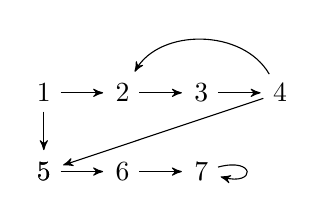
\begin{tikzpicture}[shorten >=1pt,node distance=1cm,>=stealth',auto]

		\tikzstyle{every node}=[scale=1.0]

		\node (q_1) {1};
		\node (q_2) [right of=q_1] {2};
		\node (q_3) [right of=q_2] {3};
		\node (q_4) [right of=q_3] {4};
		\node (q_5) [below of=q_1] {5};
		\node (q_6) [right of=q_5] {6};
		\node (q_7) [right of=q_6] {7};
		\node (q_5) [below of=q_1] {5};

		\path[->] (q_1) edge node {} (q_5)
					(q_1) edge node {} (q_2)
					(q_2) edge node {} (q_3)
					(q_3) edge node {} (q_4)
					(q_5) edge node {} (q_6)
					(q_6) edge node {} (q_7)
					(q_4) edge node {} (q_5)
					(q_7) edge[loop right] node {} ()
					(q_4) edge[out=120,in=60] node {} (q_2);
		\end{tikzpicture}
		\end{figure}

		\pause
		\column{.5\textwidth}
		\vspace*{-0.7cm}
		\begin{matharray}{l@{}l}
			\alert{S} \  & \Rightarrow \alert{A}BC \;[2] \\
						& \Rightarrow aA\alert{B}C \;[3] \\
						& \Rightarrow aAbB\alert{C} \;[4] \\
						& \Rightarrow a\alert{A}bBcC \;[5] \\
						& \Rightarrow aab\alert{B}cC \;[6] \\
						& \Rightarrow aabbc\alert{C} \;[7] \\
						& \Rightarrow aabbcc \;[7]
		\end{matharray}

		\pause
		\vspace*{0.5cm}
		\[
			L(G) = \{a^{n}b^{n}c^{n} \colon n \geq 1 \}
		\]
	\end{columns}
\end{frame}

\subsection{Generative Power}

\begin{frame}{Generative Power}
	\begin{center}
		\begin{figure}[!ht]
		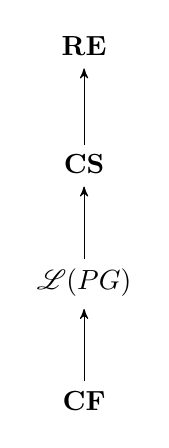
\begin{tikzpicture}[shorten >=1pt,node distance=1.4cm,>=stealth',auto]
			\tikzstyle{every node}=[scale=1.0]

			\node (CF) {\textbf{CF}};
			\node (CS) at (0, 3) {\textbf{CS}};
			\node (RE) at (0, 4.5) {\textbf{RE}};
			\node (L_{PG}) at (0, 1.5) {$\mathscr{L}(PG)$};

			\path[->]
				(CF) edge node {} (L_{PG})
				(L_{PG}) edge node {} (CS)
				(CS) edge node {} (RE);
		\end{tikzpicture}
		\end{figure}
	\end{center}
\end{frame}

\subsection{Decidable/Undecidable Problems}

\begin{frame}{Decidable/Undecidable Problems}
	\begin{center}
		\begin{table}[t]
			\centering
			\begin{tabular}{|l||c|c|c|c|}
				\hline
				Problem      & \textbf{CF} & $\mathscr{L}(PG)$ & \textbf{CS} & \textbf{RE} \\
				\hline\hline
				Membership   & $+$         &  $+$              &  $+$        & $-$ \\
				\hline
				Emptiness    & $+$         &  $+$              &  $-$        & $-$ \\
				\hline
				Equivalence  & $-$         &  $-$              &  $-$        & $-$ \\
				\hline
			\end{tabular}
		\end{table}
	\end{center}
	\begin{description}
		\item[$+$] Decidable
		\item[$-$] Undecidable
	\end{description}

\end{frame}

\section{Leftmost and $n$-limited Derivations}

\subsection{Leftmost Derivations}

\begin{frame}{Leftmost Derivations}
	\begin{description}
		\item[Idea:] At each step of a derivation the leftmost occurence of a nonterminal has to be rewritten. \\
		\bigskip
		\item[Example:] $(r: A \rightarrow v, \sigma(r))$ \\
			$w\alert{A_{1}}xA_{2}yA_{3}z \Rightarrow wvxA_{2}yA_{3}z\;[r]$ \quad(only!) \\
		\bigskip
		\item[Problem:] We decrease the generative power of programmed grammars to \textbf{CF}.
	\end{description}
\end{frame}

\subsection{$n$-limited Derivations}

\begin{frame}{$n$-limited Derivations}
	\begin{description}
		\item[Idea:] At each step of a derivation the \alert{$k$-leftmost} occurence of a nonterminal has to be rewritten,
			where \alert{$k \leq n$}. \\
		\medskip
		\item[Example:] $(r: A \rightarrow v, \sigma(r))$ \\
			$x_{0}\alert{A_{1}}x_{1}\alert{A_{2}}x_{2}\dots \alert{A_{n}}x_{n}\dots A_{n+1}x_{n+1}\dots A_{h}x_{h} \Rightarrow$
			\begin{itemize}
				\item[] $x_{0}vx_{1}A_{2}x_{2}\dots A_{n}x_{n}\dots A_{n+1}x_{n+1}\dots A_{h}x_{h}\;[r]$ or
				\item[] $x_{0}A_{1}x_{1}vx_{2}\dots A_{n}x_{n}\dots A_{n+1}x_{n+1}\dots A_{h}x_{h}\;[r]$ or
				\item[] \hspace{3cm} $\vdots$
				\item[] $x_{0}A_{1}x_{1}A_{2}x_{2}\dots vx_{n}\dots A_{n+1}x_{n+1}\dots A_{h}x_{h}\;[r]$.
			\end{itemize}
		\medskip
		\item[Question:] How does this affect the generative power?
	\end{description}
\end{frame}

\section{Infinite Hierarchy}

\begin{frame}{Infinite Hierarchy of Language Families}

\begin{center}
	\begin{figure}[!ht]
	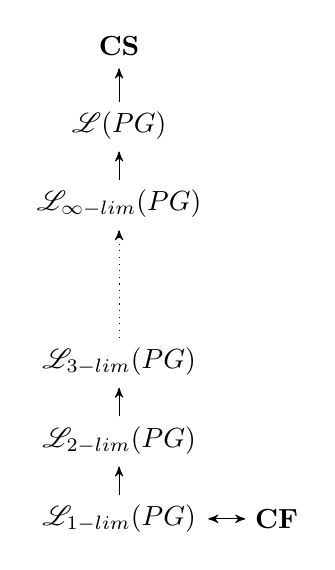
\begin{tikzpicture}[shorten >=1pt,node distance=1.4cm,>=stealth',auto]
		\tikzstyle{every node}=[scale=1.0]

		\node (CF) at (2, 0) {\textbf{CF}};
		\node (CS) at (0, 6) {\textbf{CS}};
		\node (L_{1-lim PG}) at (0, 0) {$\mathscr{L}_{\nlim{1}}(PG)$};
		\node (L_{2-lim PG}) at (0, 1) {$\mathscr{L}_{\nlim{2}}(PG)$};
		\node (L_{3-lim PG}) at (0, 2) {$\mathscr{L}_{\nlim{3}}(PG)$};
		\node (L_{inf-lim PG}) at (0, 4) {$\mathscr{L}_{\nlim{\infty}}(PG)$};
		\node (L_{PG}) at (0, 5) {$\mathscr{L}(PG)$};

		\path[<->]
			(CF) edge node {} (L_{1-lim PG});
		\path[->]
			(L_{1-lim PG}) edge node {} (L_{2-lim PG})
			(L_{2-lim PG}) edge node {} (L_{3-lim PG})
			(L_{inf-lim PG}) edge node {} (L_{PG})
			(L_{PG}) edge node {} (CS);
		\path[->, dotted]
			(L_{3-lim PG}) edge node {} (L_{inf-lim PG});
	\end{tikzpicture}
	\end{figure}
\end{center}
\end{frame}

% References
\appendix
\section<presentation>*{\appendixname}
\subsection<presentation>*{References}

\begin{frame}[allowframebreaks]
	\frametitle<presentation>{References}

	\begin{thebibliography}{10}
		\beamertemplatebookbibitems

		\bibitem{DasPau89}
		{J\"{u}rgen} Dassow and Gheorghe {P\u{a}un}
		\newblock {\em Regulated Rewriting in Formal Language Theory}.
		\newblock Springer, New York, 1989.

		\bibitem{Med00}
		Alexander Meduna
		\newblock {\em Automata and Languages: Theory and Applications}.
		\newblock Springer, London, 2000.
	\end{thebibliography}
\end{frame}

\end{document}

% End of file
